\section{Gradients and Backpropagation Basics}

This section introduces the basic notions of loss functions, gradients, and backpropagation from an abstract operator point of view. In the figures later in the document we mainly show how tensors flow along edges; the detailed Jacobian matrices are not drawn explicitly. Instead, we use a compact notation for local backward operators such as $\mathrm{d}f$, which map upstream gradients on the outputs of a node to gradients on its inputs.

\subsection{Scalar Loss and Gradient Notation}

Training a Transformer model is formulated as minimizing a scalar loss function $\mathcal{L}(\theta)$ with respect to the model parameters $\theta$. For a batch of input--target pairs $(\mathbf{X}, \mathbf{Y}_{\text{targets}})$, the model produces predictions
\[
\mathbf{Y} = f_\theta(\mathbf{X}),
\]
and a scalar loss
\[
\mathcal{L} = \mathcal{L}(\mathbf{Y}, \mathbf{Y}_{\text{targets}}).
\]

We use the differential-style notation $\mathrm{d}\theta = \partial\mathcal{L}/\partial\theta$ for gradients. For example,
\[
\mathrm{d}\mathbf{X} = \frac{\partial\mathcal{L}}{\partial\mathbf{X}}, \quad
\mathrm{d}\mathbf{W} = \frac{\partial\mathcal{L}}{\partial\mathbf{W}}, \quad
\mathrm{d}\mathbf{b} = \frac{\partial\mathcal{L}}{\partial\mathbf{b}}.
\]

In the diagrams, these gradients appear as edges labeled $\mathrm{d}\mathbf{X}$, $\mathrm{d}\mathbf{W}$, etc. together with their tensor shapes such as $[B, S, D]$ or $[D, D]$.

\subsection{Single-Input Nodes and Backward Operators}

Consider a single node in a computation graph with forward computation
\[
\mathbf{y} = f(\mathbf{x}),
\]
where $\mathbf{x}$ and $\mathbf{y}$ are vectors or tensors. Let $\mathbf{J}_f(\mathbf{x})$ denote the Jacobian of $f$ at $\mathbf{x}$. If the loss $\mathcal{L}$ depends on $\mathbf{y}$, then by the chain rule
\[
\mathrm{d}\mathbf{x} = \frac{\partial\mathcal{L}}{\partial\mathbf{x}}
= \mathbf{J}_f(\mathbf{x})^T \frac{\partial\mathcal{L}}{\partial\mathbf{y}}
= \mathbf{J}_f(\mathbf{x})^T \mathrm{d}\mathbf{y}.
\]

In the figures we do not materialize the Jacobian. Instead we introduce an \textbf{abstract backward operator} $\mathrm{d}f$ and write
\[
\boxed{\mathrm{d}\mathbf{x} = \mathrm{d}f(\mathbf{x}, \mathrm{d}\mathbf{y})},
\]
with the understanding that
\[
\mathrm{d}f(\mathbf{x}, \mathrm{d}\mathbf{y}) \equiv \mathbf{J}_f(\mathbf{x})^T \mathrm{d}\mathbf{y}.
\]

\textbf{Graphical representation:}

\begin{center}
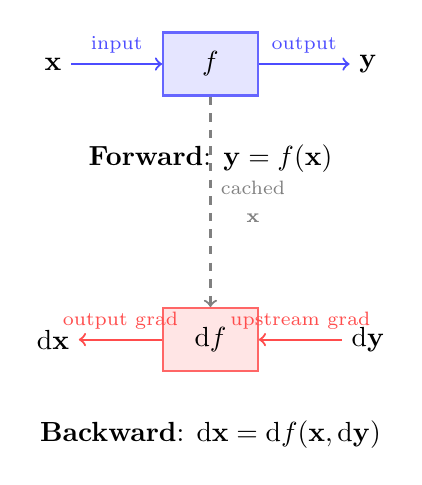
\begin{tikzpicture}[
  node distance=2cm,
  fwdnode/.style={rectangle, draw=blue!60, fill=blue!10, thick, minimum width=1.2cm, minimum height=0.8cm},
  bwdnode/.style={rectangle, draw=red!60, fill=red!10, thick, minimum width=1.2cm, minimum height=0.8cm},
  tensor/.style={},
  fwdarrow/.style={->, thick, blue!70},
  bwdarrow/.style={->, thick, red!70},
  cachearrow/.style={->, thick, dashed, gray}
]

% Forward pass
\node[tensor] (x_fwd) {$\mathbf{x}$};
\node[fwdnode, right of=x_fwd] (f_node) {$f$};
\node[tensor, right of=f_node] (y_fwd) {$\mathbf{y}$};

\draw[fwdarrow] (x_fwd) -- (f_node) node[midway, above] {\scriptsize input};
\draw[fwdarrow] (f_node) -- (y_fwd) node[midway, above] {\scriptsize output};

\node[below of=f_node, node distance=1.2cm] (fwd_label) {\textbf{Forward}: $\mathbf{y} = f(\mathbf{x})$};

% Backward pass
\node[tensor, below of=x_fwd, node distance=3.5cm] (dx_bwd) {$\mathrm{d}\mathbf{x}$};
\node[bwdnode, right of=dx_bwd] (df_node) {$\mathrm{d}f$};
\node[tensor, right of=df_node] (dy_bwd) {$\mathrm{d}\mathbf{y}$};

\draw[bwdarrow] (dy_bwd) -- (df_node) node[midway, above] {\scriptsize upstream grad};
\draw[bwdarrow] (df_node) -- (dx_bwd) node[midway, above] {\scriptsize output grad};

% Cache connection
\draw[cachearrow] (f_node) -- (df_node) node[midway, right, align=center] {\scriptsize cached\\[-2pt]\scriptsize $\mathbf{x}$};

\node[below of=df_node, node distance=1.2cm] (bwd_label) {\textbf{Backward}: $\mathrm{d}\mathbf{x} = \mathrm{d}f(\mathbf{x}, \mathrm{d}\mathbf{y})$};

\end{tikzpicture}
\end{center}

Conceptually, each backward node in the graph implements the local mapping
\[
(\mathbf{x}, \mathrm{d}\mathbf{y}) \mapsto \mathrm{d}\mathbf{x},
\]
where:
\begin{itemize}
\item \textbf{Input 1 (cached)}: The forward input $\mathbf{x}$ is cached during the forward pass
\item \textbf{Input 2 (upstream)}: The upstream gradient $\mathrm{d}\mathbf{y}$ flows from the next layer
\item \textbf{Output}: The resulting local gradient $\mathrm{d}\mathbf{x}$ flows to the previous layer
\end{itemize}

Softmax, dropout, layer normalization, and many other operators in a Transformer layer are special cases of this pattern. Their concrete backward rules are described in terms of such operators $\mathrm{d}f$.

\subsection{Nodes with Multiple Inputs}

Many nodes in a Transformer layer have several inputs. For example, a matrix multiplication node uses both an activation tensor and a weight matrix, and a layer-normalization node uses inputs as well as learned scale and shift parameters. Abstractly, we write
\[
\mathbf{y} = f(\mathbf{x}_1, \mathbf{x}_2, \ldots, \mathbf{x}_k),
\]
where each $\mathbf{x}_i$ may be a tensor of its own.

Given the upstream gradient $\mathrm{d}\mathbf{y} = \partial\mathcal{L}/\partial\mathbf{y}$, the chain rule yields gradients with respect to all inputs,
\[
\mathrm{d}\mathbf{x}_i = \mathbf{J}_{f,\mathbf{x}_i}(\mathbf{x}_1, \ldots, \mathbf{x}_k)^T \mathrm{d}\mathbf{y}, \quad i = 1, \ldots, k,
\]
where $\mathbf{J}_{f,\mathbf{x}_i}$ is the Jacobian of $f$ with respect to the $i$-th input.

We encode this in an abstract backward operator
\[
\mathrm{d}_{\mathbf{x}_i}f(\mathbf{x}_1, \ldots, \mathbf{x}_k, \mathrm{d}\mathbf{y}) := \mathbf{J}_{f,\mathbf{x}_i}(\mathbf{x}_1, \ldots, \mathbf{x}_k)^T \mathrm{d}\mathbf{y},
\]
so that, for each input,
\[
\mathrm{d}\mathbf{x}_i = \mathrm{d}_{\mathbf{x}_i}f(\mathbf{x}_1, \ldots, \mathbf{x}_k, \mathrm{d}\mathbf{y}).
\]

Collecting all input gradients together, we can also view the backward node as a single vector-valued operator
\[
\boxed{(\mathrm{d}\mathbf{x}_1, \ldots, \mathrm{d}\mathbf{x}_k) = \mathrm{d}f(\mathbf{x}_1, \ldots, \mathbf{x}_k, \mathrm{d}\mathbf{y})},
\]
whose components are exactly the individual $\mathrm{d}_{\mathbf{x}_i}f(\cdot, \ldots, \cdot, \mathrm{d}\mathbf{y})$.

\textbf{Example: Matrix Multiplication}

\begin{center}
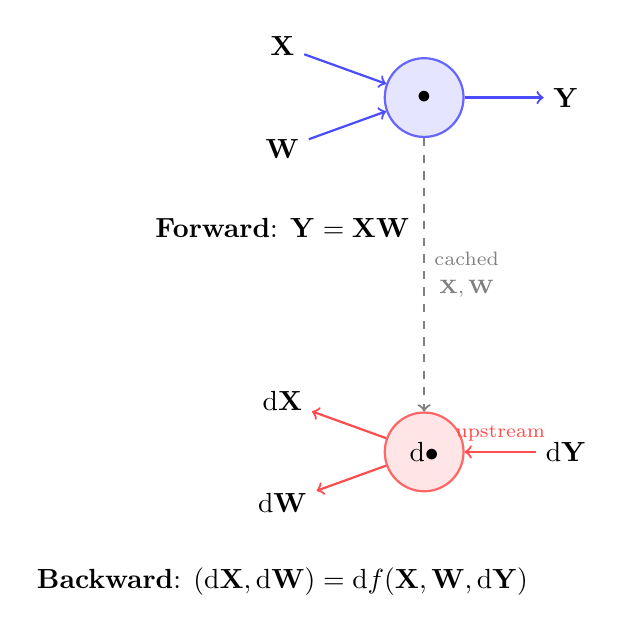
\begin{tikzpicture}[
  node distance=1.8cm,
  fwdnode/.style={circle, draw=blue!60, fill=blue!10, thick, minimum size=1cm},
  bwdnode/.style={circle, draw=red!60, fill=red!10, thick, minimum size=1cm},
  tensor/.style={},
  fwdarrow/.style={->, thick, blue!70},
  bwdarrow/.style={->, thick, red!70},
  cachearrow/.style={->, thick, dashed, gray}
]

% Forward pass
\node[tensor] (x_fwd) {$\mathbf{X}$};
\node[tensor, below of=x_fwd, node distance=1.3cm] (W_fwd) {$\mathbf{W}$};
\node[fwdnode, right of=x_fwd, yshift=-0.65cm] (f_node) {$\bullet$};
\node[tensor, right of=f_node] (y_fwd) {$\mathbf{Y}$};

\draw[fwdarrow] (x_fwd) -- (f_node);
\draw[fwdarrow] (W_fwd) -- (f_node);
\draw[fwdarrow] (f_node) -- (y_fwd);

\node[below of=W_fwd, node distance=1.0cm] (fwd_label) {\textbf{Forward}: $\mathbf{Y} = \mathbf{X}\mathbf{W}$};

% Backward pass
\node[tensor, below of=x_fwd, node distance=4.5cm] (dx_bwd) {$\mathrm{d}\mathbf{X}$};
\node[tensor, below of=W_fwd, node distance=4.5cm] (dW_bwd) {$\mathrm{d}\mathbf{W}$};
\node[bwdnode, right of=dx_bwd, yshift=-0.65cm] (df_node) {$\mathrm{d}\bullet$};
\node[tensor, right of=df_node] (dy_bwd) {$\mathrm{d}\mathbf{Y}$};

\draw[bwdarrow] (dy_bwd) -- (df_node) node[midway, above] {\scriptsize upstream};
\draw[bwdarrow] (df_node) -- (dx_bwd);
\draw[bwdarrow] (df_node) -- (dW_bwd);

% Cache connections
\draw[cachearrow] (f_node) -- (df_node) node[midway, right, align=center] {\scriptsize cached\\[-2pt]\scriptsize $\mathbf{X}, \mathbf{W}$};

\node[below of=dW_bwd, node distance=1.0cm] (bwd_label) {\textbf{Backward}: $(\mathrm{d}\mathbf{X}, \mathrm{d}\mathbf{W}) = \mathrm{d}f(\mathbf{X}, \mathbf{W}, \mathrm{d}\mathbf{Y})$};

\end{tikzpicture}
\end{center}

\vspace{0.3cm}

\noindent
\textbf{Concrete formulas:}
\begin{align*}
\mathrm{d}\mathbf{X} &= \mathrm{d}\mathbf{Y} \mathbf{W}^T \\
\mathrm{d}\mathbf{W} &= \mathbf{X}^T \mathrm{d}\mathbf{Y}
\end{align*}

In the diagrams, this is represented as a single backward node (for example, a node labeled \texttt{dMatmul} or \texttt{dLN}) with multiple incoming edges carrying the necessary forward inputs and the upstream gradient, and multiple outgoing edges carrying $\mathrm{d}\mathbf{x}_1, \ldots, \mathrm{d}\mathbf{x}_k$.

\subsection{Computation Graph and Backpropagation}

A full Transformer layer can be viewed as a composition of simpler operations:
\[
\mathbf{X}_0 \xrightarrow{f_1} \mathbf{X}_1 \xrightarrow{f_2} \mathbf{X}_2 \xrightarrow{\cdots} \mathbf{X}_L,
\]
where $\mathbf{X}_0$ is the input to the layer and $\mathbf{X}_L$ is the final output before the loss. Each $f_\ell$ is a local operator such as a matrix multiplication, a nonlinearity, a dropout, or a normalization.

Backpropagation proceeds in reverse order. Starting from $\mathrm{d}\mathbf{X}_L = \partial\mathcal{L}/\partial\mathbf{X}_L$, we apply the corresponding backward operator for each node:
\[
\mathrm{d}\mathbf{X}_\ell = \mathrm{d}f_\ell(\mathbf{X}_\ell, \mathrm{d}\mathbf{X}_{\ell+1}), \quad \ell = L-1, L-2, \ldots, 0.
\]

\textbf{Graphical representation of a computation chain:}

\begin{center}
\begin{tikzpicture}[
  node distance=1.5cm,
  fwdnode/.style={rectangle, draw=blue!60, fill=blue!10, thick, minimum width=1cm, minimum height=0.7cm},
  bwdnode/.style={rectangle, draw=red!60, fill=red!10, thick, minimum width=1cm, minimum height=0.7cm},
  tensor/.style={font=\small},
  fwdarrow/.style={->, thick, blue!70},
  bwdarrow/.style={->, thick, red!70},
  cachearrow/.style={->, thick, dashed, gray, shorten >=2pt, shorten <=2pt}
]

% Forward pass
\node[tensor] (x0) {$\mathbf{X}_0$};
\node[fwdnode, right of=x0] (f1) {$f_1$};
\node[tensor, right of=f1] (x1) {$\mathbf{X}_1$};
\node[fwdnode, right of=x1] (f2) {$f_2$};
\node[tensor, right of=f2] (x2) {$\mathbf{X}_2$};
\node[right of=x2, node distance=0.8cm] (dots) {$\cdots$};
\node[fwdnode, right of=dots, node distance=0.8cm] (fL) {$f_L$};
\node[tensor, right of=fL] (xL) {$\mathbf{X}_L$};
\node[right of=xL, node distance=1.3cm] (loss) {$\xrightarrow{\mathcal{L}}$};

\draw[fwdarrow] (x0) -- (f1);
\draw[fwdarrow] (f1) -- (x1);
\draw[fwdarrow] (x1) -- (f2);
\draw[fwdarrow] (f2) -- (x2);
\draw[fwdarrow] (x2) -- (dots);
\draw[fwdarrow] (dots) -- (fL);
\draw[fwdarrow] (fL) -- (xL);

\node[above of=x1, node distance=0.9cm, blue] {\scriptsize\textbf{Forward pass}};

% Backward pass
\node[tensor, below of=x0, node distance=2.5cm] (dx0) {$\mathrm{d}\mathbf{X}_0$};
\node[bwdnode, right of=dx0] (df1) {$\mathrm{d}f_1$};
\node[tensor, right of=df1] (dx1) {$\mathrm{d}\mathbf{X}_1$};
\node[bwdnode, right of=dx1] (df2) {$\mathrm{d}f_2$};
\node[tensor, right of=df2] (dx2) {$\mathrm{d}\mathbf{X}_2$};
\node[right of=dx2, node distance=0.8cm] (bdots) {$\cdots$};
\node[bwdnode, right of=bdots, node distance=0.8cm] (dfL) {$\mathrm{d}f_L$};
\node[tensor, right of=dfL] (dxL) {$\mathrm{d}\mathbf{X}_L$};

\draw[bwdarrow] (dx1) -- (df1);
\draw[bwdarrow] (df1) -- (dx0);
\draw[bwdarrow] (dx2) -- (df2);
\draw[bwdarrow] (df2) -- (dx1);
\draw[bwdarrow] (bdots) -- (dx2);
\draw[bwdarrow] (dxL) -- (dfL);
\draw[bwdarrow] (dfL) -- (bdots);

\node[above of=dx1, node distance=0.9cm, red] {\scriptsize\textbf{Backward pass}};

% Cache arrows
\draw[cachearrow] (f1) -- (df1);
\draw[cachearrow] (f2) -- (df2);
\draw[cachearrow] (fL) -- (dfL);

\end{tikzpicture}
\end{center}

\vspace{0.3cm}

\noindent
Key observations:
\begin{itemize}
\item \textbf{Forward}: Data flows left to right through function nodes $f_\ell$
\item \textbf{Backward}: Gradients flow right to left through backward nodes $\mathrm{d}f_\ell$
\item \textbf{Cache}: Each backward node $\mathrm{d}f_\ell$ needs access to the cached forward state $\mathbf{X}_\ell$
\item \textbf{Chain rule}: $\mathrm{d}\mathbf{X}_\ell = \mathrm{d}f_\ell(\mathbf{X}_\ell, \mathrm{d}\mathbf{X}_{\ell+1})$ for $\ell = L-1, \ldots, 0$
\end{itemize}

If $f_\ell$ depends on additional inputs (e.g. parameters), then its backward operator also produces gradients with respect to those inputs, as discussed below.

In the diagrams, we emphasize this process by drawing:
\begin{itemize}
\item \textbf{forward edges} for $\mathbf{X}_\ell$ flowing into the forward nodes $f_\ell$,
\item \textbf{backward edges} for $\mathrm{d}\mathbf{X}_\ell$ flowing out of the corresponding backward nodes $\mathrm{d}f_\ell$.
\end{itemize}

The detailed formulas that define each local operator $\mathrm{d}f_\ell$ are hidden inside the node and explained in the operator dictionary of Section 4.

\subsection{Parameter Gradients and Updates}

Parameters such as weight matrices and bias vectors enter the graph as additional inputs to some node. For example, consider a matrix multiplication
\[
\mathbf{Y} = \mathbf{X}\mathbf{W},
\]
where $\mathbf{X}$ is an activation tensor and $\mathbf{W}$ is a weight matrix. We view this as a function of two inputs,
\[
\mathbf{Y} = f(\mathbf{X}, \mathbf{W}).
\]

The corresponding backward operator produces both activation and parameter gradients:
\[
\boxed{(\mathrm{d}\mathbf{X}, \mathrm{d}\mathbf{W}) = \mathrm{d}f(\mathbf{X}, \mathbf{W}, \mathrm{d}\mathbf{Y})}.
\]

\textbf{Parameter gradient flow:}

\begin{center}
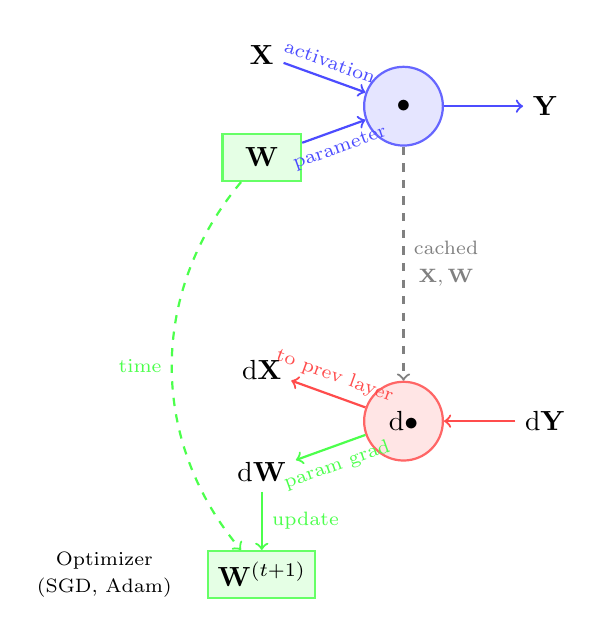
\begin{tikzpicture}[
  node distance=1.8cm,
  fwdnode/.style={circle, draw=blue!60, fill=blue!10, thick, minimum size=1cm},
  bwdnode/.style={circle, draw=red!60, fill=red!10, thick, minimum size=1cm},
  paramnode/.style={rectangle, draw=green!60, fill=green!10, thick, minimum width=1cm, minimum height=0.6cm},
  tensor/.style={},
  fwdarrow/.style={->, thick, blue!70},
  bwdarrow/.style={->, thick, red!70},
  paramarrow/.style={->, thick, green!70},
  cachearrow/.style={->, thick, dashed, gray}
]

% Forward pass
\node[tensor] (x_fwd) {$\mathbf{X}$};
\node[paramnode, below of=x_fwd, node distance=1.3cm] (W_fwd) {$\mathbf{W}$};
\node[fwdnode, right of=x_fwd, yshift=-0.65cm] (f_node) {$\bullet$};
\node[tensor, right of=f_node] (y_fwd) {$\mathbf{Y}$};

\draw[fwdarrow] (x_fwd) -- (f_node) node[midway, above, sloped] {\scriptsize activation};
\draw[fwdarrow] (W_fwd) -- (f_node) node[midway, below, sloped] {\scriptsize parameter};
\draw[fwdarrow] (f_node) -- (y_fwd);

% Backward pass
\node[tensor, below of=x_fwd, node distance=4cm] (dx_bwd) {$\mathrm{d}\mathbf{X}$};
\node[tensor, below of=W_fwd, node distance=4cm] (dW_bwd) {$\mathrm{d}\mathbf{W}$};
\node[bwdnode, right of=dx_bwd, yshift=-0.65cm] (df_node) {$\mathrm{d}\bullet$};
\node[tensor, right of=df_node] (dy_bwd) {$\mathrm{d}\mathbf{Y}$};

\draw[bwdarrow] (dy_bwd) -- (df_node);
\draw[bwdarrow] (df_node) -- (dx_bwd) node[midway, above, sloped] {\scriptsize to prev layer};
\draw[paramarrow] (df_node) -- (dW_bwd) node[midway, below, sloped] {\scriptsize param grad};

% Optimizer
\node[paramnode, below of=dW_bwd, node distance=1.3cm] (W_next) {$\mathbf{W}^{(t+1)}$};
\node[left of=W_next, node distance=2cm, align=center] (opt_label) {\scriptsize Optimizer\\[-2pt]\scriptsize (SGD, Adam)};

\draw[paramarrow] (dW_bwd) -- (W_next) node[midway, right] {\scriptsize update};
\draw[paramarrow, dashed, bend right=40] (W_fwd) to node[midway, left] {\scriptsize time} (W_next);

% Cache connections
\draw[cachearrow] (f_node) -- (df_node) node[midway, right, align=center] {\scriptsize cached\\[-2pt]\scriptsize $\mathbf{X}, \mathbf{W}$};

\end{tikzpicture}
\end{center}

\vspace{0.3cm}

\noindent
An optimizer then uses the parameter gradients to update the parameters. For example, stochastic gradient descent with learning rate $\eta$ performs
\[
\theta^{(t+1)} = \theta^{(t)} - \eta \, \mathrm{d}\theta^{(t)}.
\]

\textbf{Key distinction}:
\begin{itemize}
\item \textbf{Activation gradients} ($\mathrm{d}\mathbf{X}$): Flow to the previous layer in the backward pass
\item \textbf{Parameter gradients} ($\mathrm{d}\mathbf{W}$): Accumulated and used by the optimizer to update weights
\end{itemize}

In this document we do not draw optimizer steps in the diagrams; we only show how $\mathrm{d}\mathbf{W}$ and $\mathrm{d}\mathbf{b}$ are computed by the backward nodes.

\subsection{Connection to the Diagrams}

The detailed MHA, MLP, and output-projection figures in later sections are best read with this abstract picture in mind:
\begin{itemize}
\item Each \textbf{forward node} (e.g. \texttt{SM}, \texttt{S}, \texttt{DO}, \texttt{LN}, \texttt{matmul}) represents a mapping $\mathbf{y} = f(\mathbf{x}_1, \ldots, \mathbf{x}_k)$.
\item Each corresponding \textbf{backward node} (e.g. \texttt{dSM}, \texttt{dS}, \texttt{dDO}, \texttt{dLN}, \texttt{dMatmul}) represents the operator
\[
(\mathrm{d}\mathbf{x}_1, \ldots, \mathrm{d}\mathbf{x}_k) = \mathrm{d}f(\mathbf{x}_1, \ldots, \mathbf{x}_k, \mathrm{d}\mathbf{y}),
\]
implemented using the appropriate Jacobian-transpose formulas for that operator.
\item Edges labeled with tensors such as $\mathbf{X}$, $\mathbf{H}$, $\mathbf{Q}$, $\mathbf{K}$, $\mathbf{V}$, $\mathbf{AS}$, and their gradients $\mathrm{d}\mathbf{X}$, $\mathrm{d}\mathbf{Q}$, $\mathrm{d}\mathbf{W}$, etc., capture only the flow of data, together with compact shape annotations like $[B, S, D]$ or $[B, N_H, S, D_h]$.
\end{itemize}

In the next section we define the graphical notation and operator dictionary used in the figures, and we specialize the abstract backward operator $\mathrm{d}f$ to concrete nodes such as softmax (\texttt{S}/\texttt{dS}), scale/mask (\texttt{SM}/\texttt{dSM}), dropout (\texttt{DO}/\texttt{dDO}), and layer normalization (\texttt{LN}/\texttt{dLN}).
